\section{Approach}\label{sec:method}

To limit the complexity, we assume
each image to be a square of $m^2$ pixels, and for all patches to
be squares of the same size, $n^2$.
We formally describe our method in Sec.~\ref{sec:overview}. To summarize,
we first segment each image into patches and store them in the \texttt{patch\_dict} table, a dictionary of patches.
Only patches sufficiently different
from all the other patches in \texttt{patch\_dict} are subsequently added to the dictionary (see sec.~\ref{sec:alg}).
We describe our patch distance in sec. \ref{sec:sim} and our implementation details in \ref{sec:impl}.
Instead of storing each image explicitly, we store pointers to the patches approximating its original patches. 
Thus, during reconstruction, we simply stitch together the patches using pointers (sec.~\ref{sec:reconst}).

\subsection{Overview}
\label{sec:overview}

Our method is governed by the following parameters:
\begin{itemize}
\item $m$ - The width and height of all images.
\item $n$ - The width and height of all patches\footnote{We assume that $m \mod n$ is $0$.}.
\item $k$ - The number of images in our database.
\item $S$ - A distance function $S \colon \mathds{I}_{n \times n} \times \mathds{I}_{n \times n} \to \mathds{N}$, where we define $\mathds{I}_{n \times n}$ to be the space of all $n \times n$ image patches.  Section \ref{sec:sim} details distance measures.  The distance function should be at least a pseudometric, so $S(P_1, P_2) = 0$ if and only if patches $P_1$ and $P_2$ are the same.
\item $T$ - A distance threshold, $T \in \mathds{R}$; used as a maximum value we allow on $S$ for patch mappings.

\end{itemize}

It is worth noting that we propose a \emph{lossy} compression scheme ($T > 0$).  For the remainder of the paper, when we use the term \emph{images} we are referring to entire images from our database.  When we use the term \emph{image patches} we are referring to small $n \times n$ contiguous portions of images in our database.  When we use the term \emph{dictionary patches}, we are specifically referring to patches which we have chosen to store in our \texttt{patch\_dict} and use for compression.  Here we present an overview of our compression method; in subsequent subsections we delve into the details.

\subsection{Algorithm} \label{sec:alg}

We begin our compression algorithm by seeding \texttt{patch\_dict} with an initial set of dictionary patches.  These patches are chosen from randomly selected $n \times n$ image patches from the entire image database (see sec. \ref{sec:sample} for a discussion of this seeding strategy).   During the image insertion step, we partition each of our images into $\left(\frac{m}{n}\right)^2$ non-overlapping patches, with the intent of mapping each image patch $P_j$ to a patch in \texttt{patch\_dict}.  Thus, rather than storing the original image patch for a given image, we simply store a pointer to a patch in \texttt{patch\_dict}.  The dictionary patch we choose is the one which is closest to the image patch according to some distance metric $S$, i.e. the patch $P_{NN}$ in \texttt{patch\_dict} such that $S(P_{NN}, P_j)$ is minimized.  If $S(P_{NN}, P_j) > T$, we then store $P_j$ as a new patch in \texttt{patch\_dict} and add a pointer to this dictionary patch from the image (at the corresponding $(x,y)$ location in the image).  Algorithm \ref{alg:insert} summarizes the image insertion procedure. Assuming that our patch dictionary is a good sample of the image patches in our image database, adding additional patches should be a relative rare procedure.  We discuss how often these extra insertions are needed in sec. \ref{sec:growing_db}. Thus, the space savings come from only needing to store an effective pointer for each image patch, rather than the entire patch data.  Note that the maximum threshold on the distance of image patches and dictionary patches guarantees that each compressed image is at most $\frac{mT}{n}$ away from its original counterpart in $S$.

\begin{algorithm}
    \caption{Basic alg. to insert image $I$ into database}
    \label{alg:insert}
\begin{algorithmic}[1]
\State $Patches \leftarrow $ \texttt{Patchify}($I,n$)
\For{$P_j$ in $Patches$}
\State $P_{NN} \leftarrow $ $argmin_{P_i \in patch\_dict} \{ S(P_i, P_j) \}$
\If {$S(P_{NN}, P_j) > T$}
\State {\texttt{insert} $P_j$ into \texttt{patches}}
\EndIf
\EndFor
\vspace{3mm}
\end{algorithmic}
\end{algorithm}

With a large table of patches, finding the closest patch can be computationally expensive.  In order to speed up the search, we employ \emph{locality sensitive hashing} (LSH).  Although this softens the constraint that we always find the closest dictionary patch in \texttt{patch\_dict} for each image patch, the closest patch is still found with very high probability, and in expectation the selected patch is still very similar.  Section \ref{sec:opt} details nearest-neighbor retrieval, and alg.~\ref{alg:insert2} includes the algorithm updated to account for this optimization.
\begin{algorithm}
    \caption{Modification of alg.~\ref{alg:insert} with approximation}
    \label{alg:insert2}
\begin{algorithmic}[1]
\State $Patches \leftarrow $ \texttt{Patchify}($I,n$)
\For{$P_j$ in $Patches$}
\State $SimPat \leftarrow $\texttt{FindLikelySimilarPatches}($P_j,patch\_dict$)
\State $P_{ANN} \leftarrow $ $argmin_{P_i \in SimPat} \{ S(P_i, P_j) \}$
\If {$S(P_{ANN}, P_j) > T$}
\State {\texttt{insert} $P_j$ into \texttt{patches}}
\EndIf
\EndFor
\vspace{3mm}
\end{algorithmic}
\end{algorithm}

We will define $M \colon \mathds{I}_{n \times n}  \to \mathds{I}_{n \times n}$ to return the closest patch to $P_j$ from the set of patches returned by FindLikelySimilarPatches. $M(P_j)$ is the approximate nearest neighbor to $P_j$.
Thus, our compression problem can formally be stated as choosing a selection of image patch to dictionary patch mappings which minimizes the storage space usage of our patch table, while constraining each image tile to be at most $T$ away from its mapped patch.  In other words,

\begin{equation*}
\begin{aligned}
& \underset{patch\_dict, M}{\text{minimize}}
& & c(k, d, m, n) \\
& \text{subject to}
& & S(P_j, M(P_j)) \leq T, \; j = 1, \ldots, k\left(\frac{m}{n}\right)^2.
\end{aligned}
\end{equation*}

where $c(\cdot, \cdot, \cdot, \cdot)$ is a cost function as defined in section \ref{sec:costeval}, $d$ is the number of patches in the dictionary (i.e. $d = |patch\_dict|$), and $k,m,n$ are as defined in \ref{sec:overview}.

Given our pointer representation, we are able to construct the compressed image quite efficiently.  Given an image identifier, we iterate over all patch pointers stored with it, associated with each image location $(x,y)$.

\subsection{Patch Distance Metric}\label{sec:sim}
There are many image similarity/distance metrics that have been developed for
images (see~\cite{yasmin2013use} for a good survey), and
our method is applicable to any metric that involves Euclidean
distance over image features, its stacked color channel pixel values
being the simplest case.

For the purpose of this project, we choose to use squared Euclidean
distance over (CIE)LUV color space.
Given two $n \times n$ patches $P_i$ and $P_j$, we evaluate distance $S$
per color channel $u$ as follows:

\begin{displaymath}
S(P_i, P_j, u) = \frac{||P_i(u) - P_j(u)||^2}{n^2}
\end{displaymath}
where $||\cdot||$ denotes standard Euclidean norm.
We normalize by the dimensionality of the space to allow us to keep the
distance threshold independent of the patch size. See section \ref{sec:simthresh} for more details.  A benefit of using a Euclidean distance metric is that it allows us to use LSH to retrieve patches that are likely to be similar.


\subsection{Implementation}\label{sec:impl}
We used $postgresql$ to construct our database, and used
Java API to talk to the database from a custom executable. Locality
sensitive hashing, image segmentation and reconstruction were
all implemented in Java, and used to construct a hash table
on patches in $postgresql$.

Our code is available at:
\begin{verbatim}
https://github.com/shumash/db_project
\end{verbatim}


The $n \times n$ patches are stored as byte data in the \texttt{patch\_dict} table.
We store the patch pointers for
each image in the \texttt{patch\_pointers} table. The full schema looks as follows:

\begin{verbatim}
patch_dict(id int PRIMARY KEY,
           patch bytea);

images(id int PRIMARY KEY);

patch_pointers(img_id int REFERENCES images(id),
               patch_id int REFERENCES patch_dict(id),
               x int,
               y int);

patch_hashes(
   patch_id int PRIMARY KEY REFERENCES patch_dict(id),
   hash int);
\end{verbatim}
where \texttt{patch\_pointers.x} and \texttt{patch\_pointers.y}
refer to the left top corner location of each patch in the image.

\noindent A visualization of our schema is provided in fig.~\ref{fig:schema}.

 \begin{figure*}
%\hspace{-25mm}
\centering
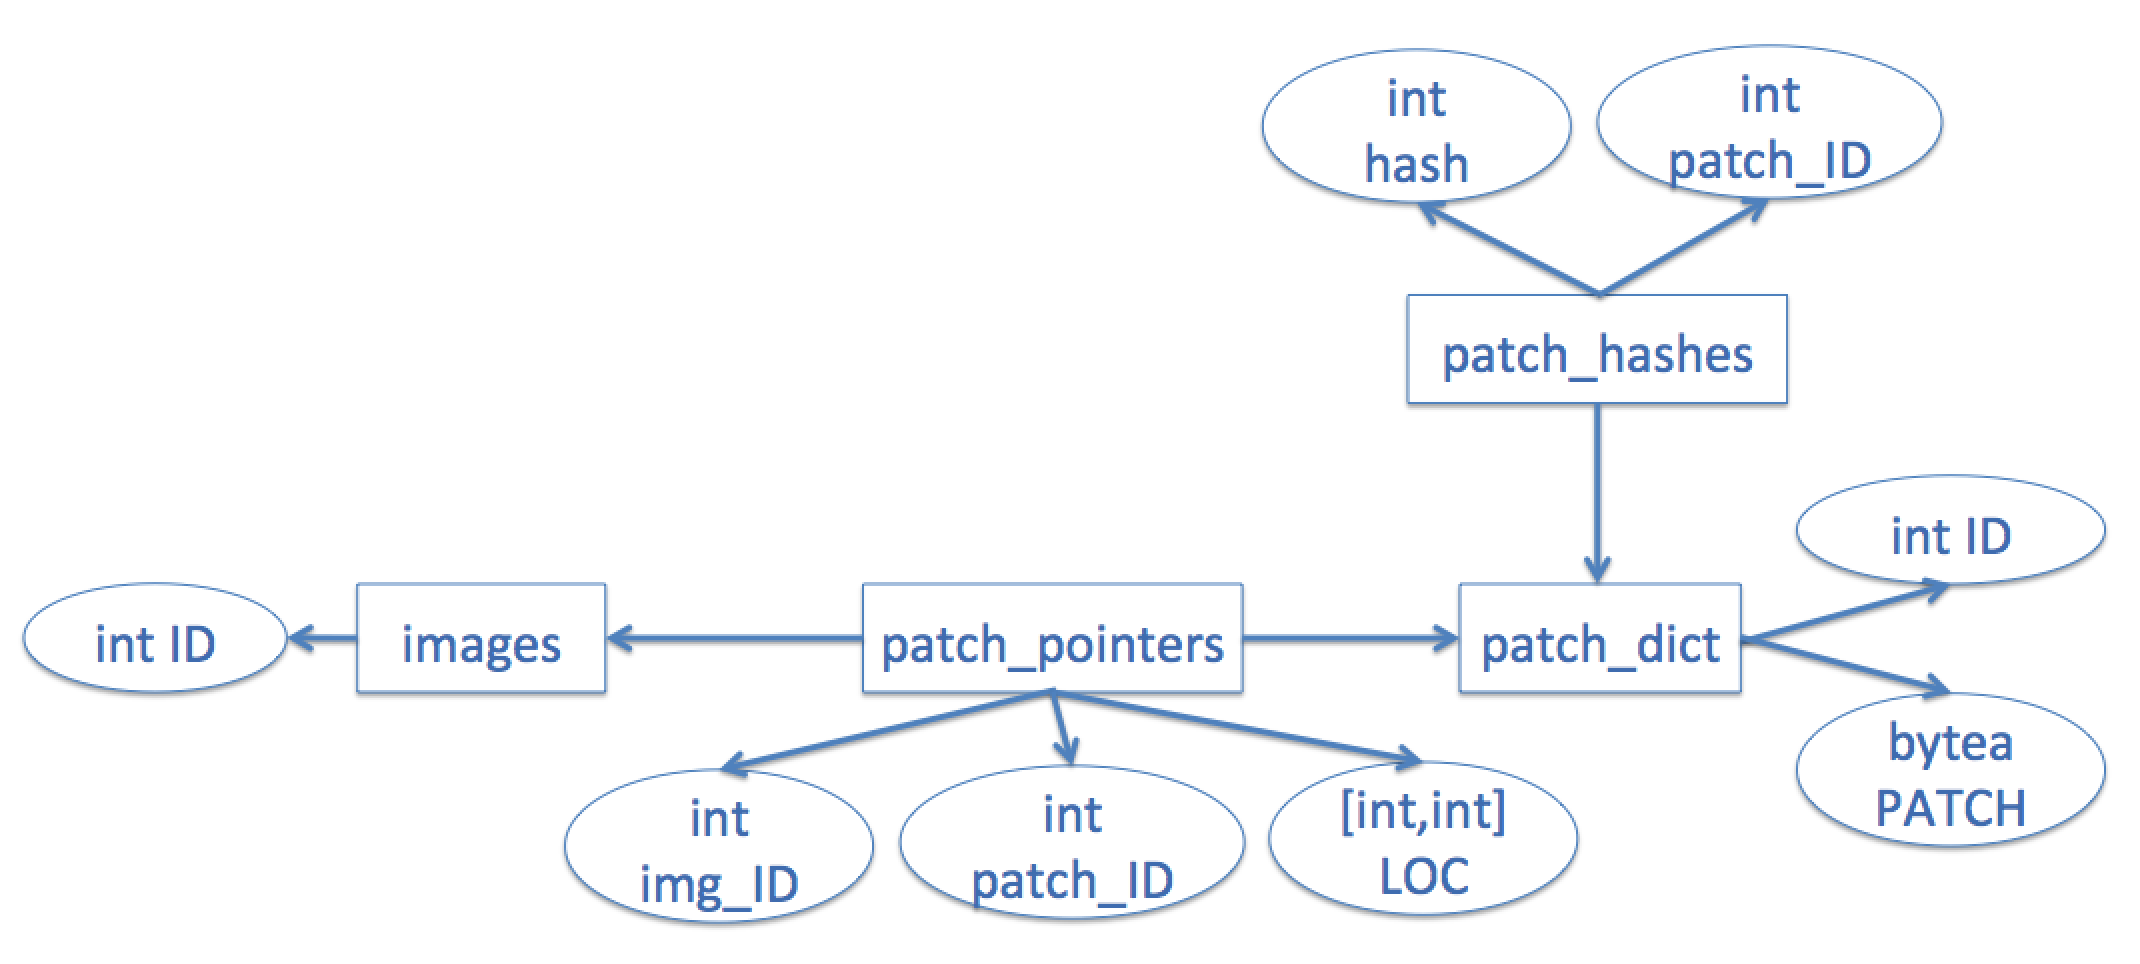
\includegraphics[width=0.6\linewidth]{Figures/ERdiagram.png}
\caption{The proposed database schema.}
\label{fig:schema}
\end{figure*}

%In order to reconstruct an image from that patches, we run the following procedure:

\subsection{Image Reconstruction}\label{sec:reconst}

To reconstruct an image, we simply follow the (logical) pointers in the corresponding \texttt{patch\_pointers} database table entry to retrieve the patches from the \texttt{patch\_dict} for each $(x,y)$ location in the image:

\begin{algorithm}
    \caption{Image reconstruction}
    \label{alg:recon}
\begin{algorithmic}[1]
\State $PatchPointers \leftarrow $ \texttt{getAllPatchPointers($patch\_pointers$)}
\State $PatchData \leftarrow $ \texttt{getAllPatches}($patch\_dict, PatchPointers$)
\State $ResultImage \leftarrow []$
\For{$P_{d}$ in $PatchData$}
\State $ResultImage.set(P_{d}.x,P_{d}.y,P_{d}.patch)$
\EndFor
\vspace{3mm}
\end{algorithmic}
\end{algorithm}



